\section{Bootprozess}

\subsection{Lerninhalt}

\begin{itemize}
   \item Sie kennen den Unterschied zwischen einer Firmware und einem Bootloader
   \item Sie kennen den Unterschied zwischen den Verzeichnissen \emph{linux/arch/<cpu>/boot} und \\ \emph{linux/init}
   \item Sie kennen die wichtigsten Dateien und Funktionen, die beim Booten eine Rolle spielen
   \item Sie kennen den Unterschied zwischen dem Real- und Protected-Mode des x86
   \item Sie kennen den Aufbau des \emph{vmlinuz}
   \item Sie kennen die Prozesse mit der PID 0 und 1
   \item Sie kennen verschiede Implementationen des Init-Programm
\end{itemize}

\subsection{Bootprozess von Linux}

\begin{figure}[h!]
   \begin{center}
      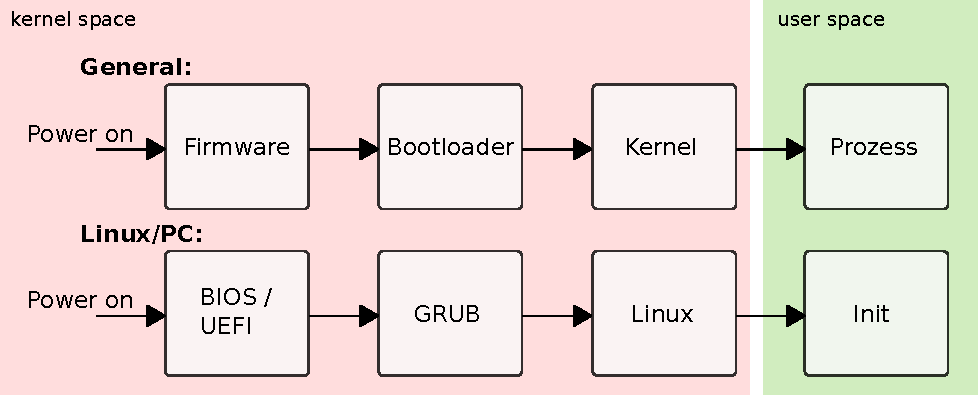
\includegraphics{images/boot_linux}
   \end{center}
   \caption{Vergleich des Bootprozess von Linux und im Allgemeinen}
   \label{fig:cmpbootlinux}
\end{figure}

Im Allgemeinen läuft beim Starten des Computers zuerst eine Art von \keyword{Firmware} (Abbildung \ref{fig:cmpbootlinux}). 
Die Firmware sucht nach der angeschlossenen \keyword{Hardware} und initialisiert diese. 
Die Firmware ist systemnah geschrieben und im System fest verankert. Anschliessend startet die 
Firmware den Bootloader oder Kernel.

\subsection{BIOS / UEFI}

Beim \keyword{Personal Computer (PC)} gibt es, ähnlich einer Firmware, das 
\keyword{Binary Input Output System (BIOS)}. Nach erfolgreichem \keyword{Power On Self Test (POST)},
lädt das BIOS die ersten 512 Bytes von der Festplatte in den Arbeitsspeicher und führt diesen aus. \\

Dieser Bereich auf der Festplatte wird \emph{Master Boot Record (MBR)}\index{Master Boot Record (MBR)} genannt.
Dieses Vorgehen ist fest im BIOS einprogrammiert und beschränkt die zu erst gestartete Software auf nur 446 Bytes,
wie in Abbildung \ref{fig:mbr} zu sehen ist. Der restliche Platz wird für die Partitionstabelle und die Bootsignatur
verwendet. Der Aufbau der Partitionstabelle beschränkt den PC auf maximal vier physikalische \keyword{Partitionen}. 
Werden trotzdem mehr Partitionen auf der Festplatte gewünscht, müssen diese über logische Partitionen realisiert werden.  \\

\begin{wrapfigure}{r}{0.40\textwidth}
   \begin{center}
      \vspace{-0.5cm}
      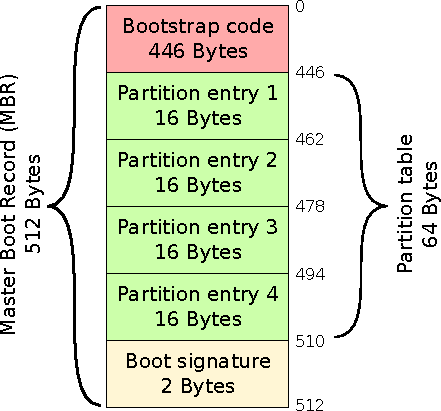
\includegraphics{images/mbr}
   \end{center}
   \caption{Aufbau des MBRs}
   \label{fig:mbr}
\end{wrapfigure}


Der Linux-Kernel befindet sich in der Grössenordnung von mehreren Megabytes und passt somit nicht in den MBR.
Aus diesem Grund wird ein \keyword{Bootloader} in den MBR geschrieben.

Bei neueren Systemen kommt anstelle des BIOS das \keyword{Unified Extensible Firmware Interface (UEFI)} zum Einsatz. Das UEFI hebt einige
Einschränkungen des BIOS auf. Es erlaubt grössere und mehr Partitionen. Auch das Problem mit dem 512-Byte grossen MBR wird dadurch gelöst.
Somit ist es auch möglich Linux, ohne Booloader zu starten. Trotzdem wird Linux oft weiterhin per Bootloader gestartet. 

\subsection{Bootloader}

Um Linux zu starten wird meistens der \keyword{GRUB}-Bootloader\footnote{\url{https://www.gnu.org/software/grub/}} 
verwendet. GRUB ermöglicht es über ein Auswahlmenü beim Booten zwischen mehreren Betriebssystemen auf einem PC zu wählen.
Ausserdem kann man mit diesem Menü den Linux-Kernel mit verschiedenen Bootparameter starten, was zum Beispiel für die
Systemwiederherstellung interessant ist.

\subsection{Kernel}

Bei Unix-Kerneln und deren Derivate werden traditionell nach Abschluss der Hardware-Initialisierung
die internen Datenstrukturen aufgebaut um die Prozess- und Speicherverwaltung zu ermöglichen.
Danach wird der \keyword{Init}-Prozess gestartet. Der Init-Prozess ist der erste
Prozess überhaupt und befindet sich überlicherweise unter \emph{/sbin/init}.

\subsection{Innerhalb des Linux-Kernels}

Die Funktionsaufrufe innerhalb des Linux-Kernels lassen sich in zwei Kategorieren einteilen. Die 
architekturspezifischen und die plattformübergreifenden Funktionsaufrufe. Um möglichst viel Code
auf allen CPU-Architekturen wiederzuverwenden, befindet sich dieser unter \emph{linux/init}.
Davor läuft immer der plattformabhängige Code, welcher pro CPU unter \emph{linux/arch/<cpu>/} zu finden
ist. Die Abbildung \ref{linux_boot} zeigt die Reihenfolge einiger wichtigen Funktionsaufrufe beim Start
des Kernels.

\clearpage

\begin{figure}[h!]
   \begin{center}
      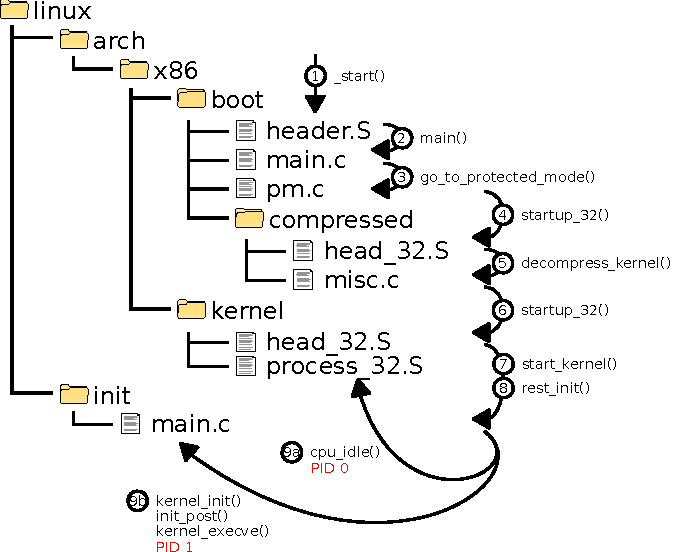
\includegraphics{images/linux_boot}
   \end{center}
   \caption{Wichtige Funktionsaufrufe innerhalb des Kernels}
   \label{linux_boot}
\end{figure}


\subsubsection{Erster Funktionsaufruf}

Wie bereits weiter oben erwähnt, ruft der Bootloader den Kernel auf. Der erste Funktionsaufruf innerhalb des Kernel ist
immer plattformabhängig, um den \keyword[Virtual Memory (VM)]{virtuellen Adressbereich} aufzusetzen, den Betriebsmode
der CPU auszuwählen und alle Prozessorkerne zu konfigurieren. Aus diesem Grund ist der erste Funktionsaufruf pro Architektur
unterschiedlich. Hier wird der Bootvorgang für die Intel x86 und deren kompatieble Prozessoren beschrieben. Der Bootvorgang
für andere CPUs ist jedoch vergleichbar und in den anderen Verzeichnissen unter \emph{linux/arch} zu finden. \\

Die Entwickler des Linux-Kernels versuchen möglichst viele Dinge in der \keyword{Programmiersprache C} zu schreiben. Hardwareeinstellungen
erfordern jedoch speziefische Operationen und daher sind diese in \keyword{Assembly} geschrieben, wie die Dateiendung \emph{.S} vermuten
lässt. Der erste Funktionsaufruf ist ebenfalls in Assembly geschrieben, wie im Listing \ref{firstcall} zu sehen ist.

\begin{lstlisting}[label=firstcall,caption=linux/arch/x86/boot/header.S]
_start:
             # Explicitly enter this as bytes, or the assembler
             # tries to generate a 3-byte jump here, which causes
             # everything else to push off to the wrong offset.
             .byte   0xeb            # short (2-byte) jump
             .byte   start_of_setup-1f

             # [..]

start_of_setup:
             # [..]

             # Jump to C code (should not return)
             calll   main
\end{lstlisting}

Zu Beginn wird die Funktion \emph{\_start()} aufgerufen, welche gleich zum Label \emph{start\_of\_setup} springt. Im Linux-Kernel trifft
man oft auf \keyword[Hack]{Hacks} oder \keyword[Workaround]{Workarounds}, um ein gewisses Verhalten explizit zu fordern. Wie der Kommentar
deutlich macht, umgeht man hier die Optimierung des \keyword[Assembler]{Assemblers}, indem man direkt den Maschienencode hexadezimal eingibt.
Die beiden Zeilen entsprechen jedoch einem simplen Jump-Befehl:
\begin{lstlisting}
jmp start_of_setup
\end{lstlisting}

Die Funktion \emph{start\_of\_setup} führt einige Checks durch, bis am Ende die C-Funktion \emph{main()} aufruft.

\subsubsection{x86-Initialisierung}

Die x86-Initialisierung passiert in der Funktion \emph{main()}, wie das Listing \ref{x86init} zeigt.

\begin{lstlisting}[label=x86init,caption=linux/arch/x86/boot/main.c]
void main(void)
{
        /* First, copy the boot header into the "zeropage" */
        copy_boot_params();

        /* Initialize the early-boot console */
        console_init();
        if (cmdline_find_option_bool("debug"))
                puts("early console in setup code\n");

        /* End of heap check */
        init_heap();

        /* Make sure we have all the proper CPU support */
        if (validate_cpu()) {
                puts("Unable to boot - please use a kernel appropriate "
                     "for your CPU.\n");
                die();
        }

        /* Tell the BIOS what CPU mode we intend to run in. */
        set_bios_mode();

        /* Detect memory layout */
        detect_memory();

        /* Set keyboard repeat rate (why?) */
        keyboard_set_repeat();

        /* Query MCA information */
        query_mca();

        /* Query Intel SpeedStep (IST) information */
        query_ist();

        /* [..] */

        /* Set the video mode */
        set_video();

        /* Do the last things and invoke protected mode */
        go_to_protected_mode();
}
\end{lstlisting}

Zuerst werden die Bootparameter gesichert. Die Bootparameter sind vergleichbar mit den Parametern in der Commandline bei einem
Programmstart. Diese ermöglichen es, beim \clearpage Booten verschiedene Optionen mitzugeben. Zum Beispiel das \keyword{Userspace}-Programm,
welches als erstes ausgeführt werden soll (üblicherweise \emph{init}) oder das Loglevel. Anschliessend wird eine Console per
Serialanschluss initialisiert, die Heap-Speichergrösse ermittelt, überprüft ob die CPU alle notwendigen Features unterstützt,
der Prozessormode per BIOS eingestellt, das Speicherlayout ausgelesen, die Tastaturwiederholungsrate gesetzt, ein
Machine Check Architecture (MCA; eine Möglichkeit der CPU dem Betriebssystem Hardwaredefekte mitzuteilen) durchgeführt, Unterstüztung 
für die Speedstep-Technologie abgefragt und der Bildschirm in den VGA-Mode geschalten. \\

Zuletzt wird die Funktion \emph{go\_to\_protected\_mode()} aufgerufen.

\subsubsection{Vom Real- zu Protected-Mode}

Der gesamte bisherige Code ist im alten 16-Bit-Modus gelaufen, dem sogenannten \keyword{Real-Mode}. Alle heutigen x86- und ia64-Prozessoren
besitzen immer noch eine volle Implementation des Befehlsatzes, der 1975 mit dem ersten Intel 8086 veröffentlicht wurde. Aus diesem Grund
ist es heutzutage immer noch möglich, ein MS-DOS auf diesen Computern zu installieren. Der Prozessor startet immer im Real-Mode und muss erst
in den 32-Bit-Modus versetzt werden, dem \keyword{Protected-Mode}. Der Protected-Mode verfügt im Gegensatz zum Real-Mode auch über eine
virtuelle Speicherverwaltung inklusive Paging. \\

\begin{figure}[h!]
   \begin{center}
      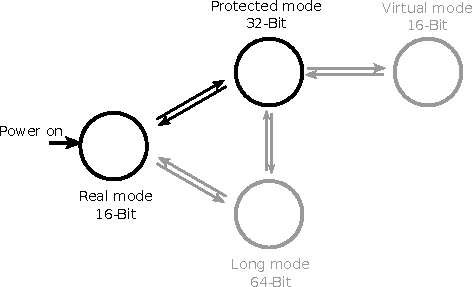
\includegraphics{images/x86modes}
   \end{center}
   \caption{Prozessor-Modes für Intel x86 kompatible CPUs}
   \label{x86modes}
\end{figure}

In Abbildung \ref{x86modes} sind noch zwei weitere Modes zu sehen. Der \keyword{Long-Mode} ist der 64-Bit-Modus und auch der Grund, warum es
möglich ist, auf dem selben Prozessor ein 32-Bit wie auch ein 64-Bit Betriebsystem zu installieren. Der \keyword{Virtual-Mode} ermöglicht 
es, Real-Mode-Programme unter einem 32-Bit Betriebssystem zu verwenden und wurde hauptsächlich in der Übergangsphase von 16- zu 32-Bit verwendet. \\

Der Code für die Umschaltung befindet sich in \emph{linux/arch/x86/boot/compressed/head\_32.S} und wird aufgrund ihrer Komplexität hier
nicht weiter behandelt. Im Protected-Mode wird die Funktion \emph{decompres\_kernel()} aufgerufen.

\subsubsection{Dekompression}

Der grösste Teil des Kernels ist mittels \keyword{zlib}, \keyword{LZMA} oder \keyword{Bzip2} komprimiert. Der komprimierte Kernel wird in dieser
Bootphase entpackt und ausgeführt. Zum einen braucht der komprimierte Kernel weniger Speicherplatz und zum anderen ist es oft schneller,
einen kleinen Kernel von der Disk zu lesen und zu dekomprieren, anstatt ein grosses Images zu lesen. Der Aufbau des Image zeigt die Abbildung \ref{vmlinuz}.

\begin{figure}[h!]
   \begin{center}
      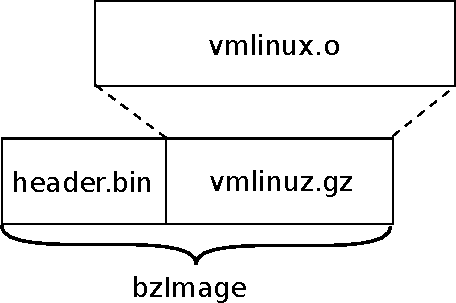
\includegraphics{images/bzimage}
   \end{center}
   \caption{Aufbau des bzImages}
   \label{vmlinuz}
\end{figure}

\begin{description}
   \item[header.bin] 
      Maschinencode, der direkt vom Bootloader ausgeführt wird, inklusive des Dekomprimierungsalgorithmus.

   \item[vmlinuz]
      Der komprimierte Kernel.

\end{description} 

\subsubsection{Start des Kernels}

Der erste Funktionsaufruf innerhalb des Kernels findet in der Assemblydatei \emph{linux/arch/x86/kernel/head\_32.S} statt.
Nach Abschluss wird die zentrale Kernel-Initialisierung gestartet, \emph{start\_kernel()}. Das Listing \ref{start_kernel} zeigt einen kurzen
Ausschnitt dieser Funktion.

\begin{lstlisting}[label=start_kernel,caption=linux/init/main.c]
asmlinkage void __init start_kernel(void)
{
        /* [..] */

        /*
         * Set up the scheduler prior starting any interrupts (such as the
         * timer interrupt). Full topology setup happens at smp_init()
         * time - but meanwhile we still have a functioning scheduler.
         */
        sched_init();
        /*
         * Disable preemption - early bootup scheduling is extremely
         * fragile until we cpu_idle() for the first time.
         */
        preempt_disable();

        /* [..] */

        early_irq_init();
        init_IRQ();
        prio_tree_init();
        init_timers();
 
        /* [..] */

        check_bugs();

        acpi_early_init(); /* before LAPIC and SMP init */
        sfi_init_late();

        ftrace_init();

        /* Do the rest non-__init'ed, we're now alive */
        rest_init();
}
\end{lstlisting}

Wie im Listing ersichtlich, startet die Funktion das Scheduling von Prozessen. Der aktuelle Prozess
trägt die \keyword{Prozess-ID (PID)} 0. In \emph{rest\_init} wird der Prozess mit der ID 1 
gestartet, welcher schliesslich das erste Userspace-Programm ausführen wird.


\begin{lstlisting}[label=start_kernel,caption=linux/init/main.c]
static noinline void __init_refok rest_init(void)
{
        int pid;

        rcu_scheduler_starting();
        /*
         * We need to spawn init first so that it obtains pid 1, however
         * the init task will end up wanting to create kthreads, which, if
         * we schedule it before we create kthreadd, will OOPS.
         */
        kernel_thread(kernel_init, NULL, CLONE_FS | CLONE_SIGHAND);
        numa_default_policy();
        pid = kernel_thread(kthreadd, NULL, CLONE_FS | CLONE_FILES);
        rcu_read_lock();
        kthreadd_task = find_task_by_pid_ns(pid, &init_pid_ns);
        rcu_read_unlock();
        complete(&kthreadd_done);

        /*
         * The boot idle thread must execute schedule()
         * at least once to get things moving:
         */
        init_idle_bootup_task(current);
        preempt_enable_no_resched();
        schedule();

        /* Call into cpu_idle with preempt disabled */
        preempt_disable();
        cpu_idle();
}
\end{lstlisting}

Der erste Prozess (PID 0) wird am Ende in den Schlafzustand versetzt (Idle). Zuvor wird der neue Prozess
mit \emph{kernel\_thread()} gestartet.

\subsection{Init}

Init steht für \emph{Initialisierung} und bezeichnet das erste Programm das gestartet wird. Bei Linux kann
dieses über Bootparameter definiert werden. Für GRUB2 kann diese unter \emph{/etc/default/grub} editiert werden:

\begin{lstlisting}[caption=/etc/default/grub]
GRUB_CMDLINE_LINUX_DEFAULT="init=/sbin/init"
\end{lstlisting}

Das ursprüngliche Init-Programm von Unix wird unter Linux nicht verwendet. Stattdessen gibt es eine Reihe von
alternativen Init-Implementationen. Die Bekannteste wird \keyword{SysV-Init} genannt und ist ziemlich simpel.
Die Textdatei \emph{/etc/initab} besitzt eine Liste von Programmen, die sequentiell gestartet werden. Neuere
Init-Implementationen versuchen über Abhängigkeiten die Prozesse parallel zu starten, um einen schnelleren
Bootvorgang zu erreichen. Die Bekannsten sind Gentoo's \keyword{OpenRC}, Ubuntu's \keyword{Upstart} und
Redhats \keyword{Systemd}.

\subsection{Zusammenfassung}

\begin{itemize}
   \item Sie kennen den Unterschied zwischen einer Firmware und einem Bootloader
   \item Sie kennen den Unterschied zwischen den Verzeichnissen \emph{linux/arch/<cpu>/boot} und \\ \emph{linux/init}
   \item Sie kennen die wichtigsten Dateien und Funktionen, die beim Booten eine Rolle spielen
   \item Sie kennen den Unterschied zwischen dem Real- und Protected-Mode des x86
   \item Sie kennen den Aufbau des \emph{vmlinuz}
   \item Sie kennen die Prozesse mit der PID 0 und 1
   \item Sie kennen verschiede Implementationen des Init-Programms
\end{itemize}

\summary{
Die Bootreihenfolge von Linux ist BIOS, Bootloader, Linux-Kernel, Init. \\

Der MBR ist 512-Bytes gross und beinhaltet den Bootloader. \\

Unter linux/arch/<cpu>/boot ist der prozessorabhängige Bootcode.\\

Unter linux/init/ ist der prozessorunabhängige Bootcode. \\

Der x86-Prozessor besitzt die Betriebszustände Real, Protected, Long und Virtual Modes. \\

Das Image des Linux-Kernels besteht aus dem Bootstrapcode und dem komprimierten Kernel. Beim
Booten entpackt der Bootstrapcode den Kernel und führt diesen aus. \\

Die bekanntesten Init-Implementationen sind SysV-Init, Systemd, Upstart und OpenRC.
}

\subsection{Diskussion}

\begin{itemize}
   \item Wieso wird Linux beim Einsatz von UEFI oft trotzdem noch über ein Bootloader gestartet?
   \item Weshalb besitzen heutige x86-Prozessoren immer noch einen Real-Mode?
   \item Wieso wird der Linux-Kernel erst beim Booten dekomprimiert? Welchen Einfluss denken Sie, hat das auf Grösse und Geschwindigkeit? 
   \item Warum wird das Init-Programm nicht aus dem Prozess mit PID 0 gestartet? PID 0 wechselt ja direkt in den Idle-Mode.
   \item Was sind die Vor- und Nachteile von SysV-Init, OpenRC, Upstart und Systemd? Welches würden Sie bevorzugen?
\end{itemize}

